\chapter{Atividades desenvolvidas}
\label{cap:atividades-desenvolvidas}

As atividades desenvolvidas durante o período do Estágio Supervisionado são descritas nesta seção. Primeiramente, uma aplicação construída para migrar dados de uma banco para outro por meio da linguagem Java é descrita, fazendo uso de conceitos apresentados na Seção~\ref{sec:java}. Posteriormente, um projeto utilizando o \textit{framework} Angular é apresentado, fazendo uso dos conceitos de UI/UX apresentados na Seção~\ref{sec:ui-e-ux}.

\section{Migração de bancos de dados em Java}
\label{sec:java-atividades}

O Avenue Code Events Billing Administration (AC-EBA) é um projeto interno da empresa que visa o gerenciamento de gastos monetários e de pessoal em eventos realizados pela Avenue Code. Originalmente desenvolvido na filial de São Paulo, uma segunda versão do sistema começou a ser projetada a fim de adicionar funcionalidades e melhorar o seu desempenho. A nova versão do AC-EBA começou a ser construída com novas linguagens de \textit{backend} e \textit{frontend} e, portanto, não foi desenvolvida sobre o código da primeira versão. Dessa forma, era necessário migrar os dados da primeira versão para a segunda, e optou-se por construir uma aplicação em Java para auxiliar nesse processo.

O Java Database Connectivity (JDBC) é uma \textit{application programming interface} (API) da linguagem da Java que possibilita gerenciar banco de dados relacionais por meio da abstração da implementação de bancos de dados específicos, criando uma camada intermediária com diversos métodos para o estabelecimento de conexões, leitura, escrita de dados, e extração de resultados a partir de \textit{queries}. Utilizando diversos métodos providos pelo JDBC, uma aplicação para a migração dos dados do banco da primeira versão do AC-EBA foi desenvolvida, e a ela foi dado o nome de AC JDB Migrator (AC-JDBM).

O AC-JDBM foi projetado em uma \textit{pipeline} de quatro etapas diferentes, mostradas na Figura~\ref{fig:java-jdbm}. As etapas da \textit{pipeline} dessa aplicação são: (i) conectar-se ao banco de dados do projeto original, (ii) ler os dados presentes nesse banco, (iii) transformar os dados de acordo com as tabelas presentes no novo sistema, e (iv) utilizar esses dados transformados para a escrita das \textit{queries} para popular o banco de dados do novo sistema.

\begin{figure}[htb!]
  \centering
  \caption{Esquema de execução da aplicação AC JDB Migrator.}
  \label{fig:java-jdbm}
  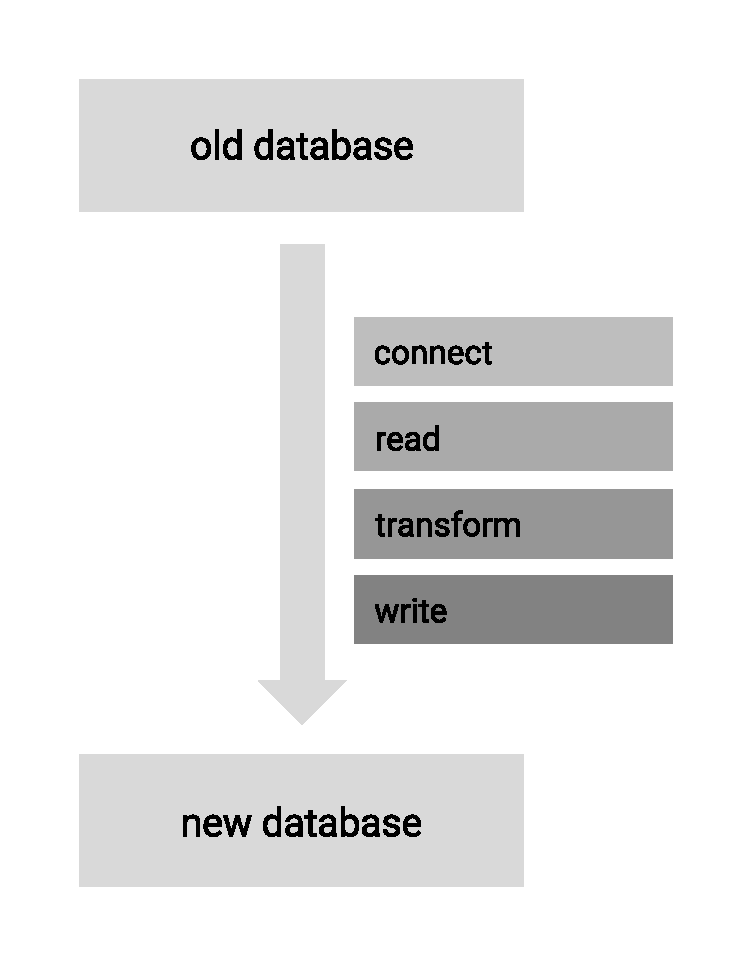
\includegraphics[width=200pt, keepaspectratio=true]{img/java-jdbm}
  \fonte{Próprio autor.}
\end{figure}

A primeira etapa da aplicação é constituída pela classe \verb|DbConnector|, que busca realizar uma conexão com um banco de dados. Para isso, ela recebe um arquivo de extensão \verb|Property| como parâmetro, que contém as credenciais necessárias para a conexão com um banco. A classe foi feita de modo genérico, sendo que é possível criar um objeto para conectar-se tanto com o banco de dados original quanto o do novo sistema, e métodos de conexão do JDBC foram utilizados em seu desenvolvimento.

A etapa seguinte corresponde à leitura dos dados do banco original, sendo realizada pela classe \verb|DbReader|. \textit{Queries} para a leitura de todas as tabelas presentes no banco original (por exemplo, \verb|select * from EVENT|) foram codificadas, e os resultados dessas \textit{queries} é obtido por meio de objetos do tipo \verb|ResultSet|. Esses objetos foram então mapeados para objetos do tipo \verb|Table|, que correspondiam às tabelas do antigo banco de dados. A classe \verb|Table| é constituída de um \verb|Set| de objetos do tipo \verb|Row|, e tanto \verb|Table| quanto \verb|Row| foram criados para armazenar os dados lidos de acordo com a tabela correspondente e, posteriormente, passá-los para a próxima etapa da \textit{pipeline}.

A terceira etapa consiste na transformação dos dados lidos para se adequarem às tabelas do banco de dados do novo projeto. O \verb|DbTransformer| foi desenvolvido para receber o conjunto de objetos do tipo \verb|Table| correspondente às tabelas do antigo banco, e transformar os dados recebidos de acordo com as tabelas no novo sistema, que diferiam do sistema original por meio da adição e/ou remoção de algumas colunas, por exemplo. Dessa forma, o \verb|DbTransformer| é constituído de outros objetos, como \verb|EventTransformer| ou \verb|BudgetTransformer|, e cada um deles retorna objetos do tipo \verb|Set| contendo uma interface construída para armazenar os dados transformados, a \verb|SQLWritable|.

Finalmente, a última etapa da \textit{pipeline} de migração do dados é responsável por conectar-se ao banco do novo sistema e escrever as \textit{queries} para a inserção dos dados transformados. Para realizar a conexão, foi utilizada uma instância do \verb|DbConnector| com um arquivo \verb|Property| com os dados do banco do novo sistema, e a interface \verb|SQLWritable| teve o método \verb|toSQL()| implementado em cada uma de suas instâncias. Esse método era responsável por escrever as \textit{queries} para a inserção dos dados de cada uma das tabelas lidas para as novas tabelas.

No desenvolvimento do AC-JDBM foram utilizados diversos conceitos de orientação a objetos, de padrões de projeto e boas práticas de programação.  A criação do projeto como uma \textit{pipeline}, a manipulação de interfaces ao invés de tipos concretos, o encapsulamento dos dados e a separação de responsabilidades pelas classes ao longo do projeto são algumas das características que contribuíram não só para o sucesso da aplicação, mas também para o aprendizado do autor na utilização da linguagem Java aplicada ao \textit{backend} de sistemas.

\section{Desenvolvimento de interfaces e experiências de usuário}
\label{sec:ui-ux-atividades}

A ser escrita.